% Für Bindekorrektur als optionales Argument "BCORfaktormitmaßeinheit", dann
% sieht auch Option "twoside" vernünftig aus
% Näheres zu "scrartcl" bzw. "scrreprt" und "scrbook" siehe KOMA-Skript Doku
\documentclass[12pt,a4paper,titlepage,headinclude,bibtotoc]{scrartcl}


%---- Allgemeine Layout Einstellungen ------------------------------------------

% Für Kopf und Fußzeilen, siehe auch KOMA-Skript Doku
\usepackage[komastyle]{scrpage2}
\pagestyle{scrheadings}
\setheadsepline{0.5pt}[\color{black}]
\automark[section]{chapter}


%Einstellungen für Figuren- und Tabellenbeschriftungen
\setkomafont{captionlabel}{\sffamily\bfseries}
\setcapindent{0em}


%---- Weitere Pakete -----------------------------------------------------------
% Die Pakete sind alle in der TeX Live Distribution enthalten. Wichtige Adressen
% www.ctan.org, www.dante.de

% Sprachunterstützung
\usepackage[ngerman]{babel}

% Benutzung von Umlauten direkt im Text
% entweder "latin1" oder "utf8"
\usepackage[utf8]{inputenc}

% Pakete mit Mathesymbolen und zur Beseitigung von Schwächen der Mathe-Umgebung
\usepackage{latexsym,exscale,stmaryrd,amssymb,amsmath}

% Weitere Symbole
\usepackage[nointegrals]{wasysym}
\usepackage{eurosym}

% Anderes Literaturverzeichnisformat
%\usepackage[square,sort&compress]{natbib}
\usepackage{hyperref}
% Für Farbe
\usepackage{color}

% Zur Graphikausgabe
%Beipiel: \includegraphics[width=\textwidth]{grafik.png}
\usepackage{graphicx}

% Text umfließt Graphiken und Tabellen
% Beispiel:
% \begin{wrapfigure}[Zeilenanzahl]{"l" oder "r"}{breite}
%   \centering
%   \includegraphics[width=...]{grafik}
%   \caption{Beschriftung} 
%   \label{fig:grafik}
% \end{wrapfigure}
\usepackage{wrapfig}

% Mehrere Abbildungen nebeneinander
% Beispiel:
% \begin{figure}[htb]
%   \centering
%   \subfigure[Beschriftung 1\label{fig:label1}]
%   {\includegraphics[width=0.49\textwidth]{grafik1}}
%   \hfill
%   \subfigure[Beschriftung 2\label{fig:label2}]
%   {\includegraphics[width=0.49\textwidth]{grafik2}}
%   \caption{Beschriftung allgemein}
%   \label{fig:label-gesamt}
% \end{figure}
\usepackage{subfigure}

% Caption neben Abbildung
% Beispiel:
% \sidecaptionvpos{figure}{"c" oder "t" oder "b"}
% \begin{SCfigure}[rel. Breite (normalerweise = 1)][hbt]
%   \centering
%   \includegraphics[width=0.5\textwidth]{grafik.png}
%   \caption{Beschreibung}
%   \label{fig:}
% \end{SCfigure}
\usepackage{sidecap}

% Befehl für "Entspricht"-Zeichen
\newcommand{\corresponds}{\ensuremath{\mathrel{\widehat{=}}}}
% Befehl für Errorfunction
\newcommand{\erf}[1]{\text{ erf}\ensuremath{\left( #1 \right)}}

%Fußnoten zwingend auf diese Seite setzen
\interfootnotelinepenalty=1000

%Für chemische Formeln (von www.dante.de)
%% Anpassung an LaTeX(2e) von Bernd Raichle
\makeatletter
\DeclareRobustCommand{\chemical}[1]{%
  {\(\m@th
   \edef\resetfontdimens{\noexpand\)%
       \fontdimen16\textfont2=\the\fontdimen16\textfont2
       \fontdimen17\textfont2=\the\fontdimen17\textfont2\relax}%
   \fontdimen16\textfont2=2.7pt \fontdimen17\textfont2=2.7pt
   \mathrm{#1}%
   \resetfontdimens}}
\makeatother

%Honecker-Kasten mit $$\shadowbox{$xxxx$}$$
\usepackage{fancybox}

%SI-Package
\usepackage{siunitx}

%keine Einrückung, wenn Latex doppelte Leerzeile
\parindent0pt

%Bibliography \bibliography{literatur} und \cite{gerthsen}
%\usepackage{cite}
\usepackage{babelbib}
\selectbiblanguage{ngerman}

\begin{document}

\begin{titlepage}
\centering
\textsc{\Large Anfängerpraktikum der Fakultät für
  Physik,\\[1.5ex] Universität Göttingen}

\vspace*{3cm}

\rule{\textwidth}{1pt}\\[0.5cm]
{\huge \bfseries
  Fresnelsche Formeln\\[1.5ex]
  und Polarisation}\\[0.5cm]
\rule{\textwidth}{1pt}

\vspace*{3cm}

\begin{Large}
\begin{tabular}{ll}
Praktikant: &  Michael Lohmann\\
Versuchspartner: &  Felix Kurtz\\
 E-Mail: & m.lohmann@stud.uni-goettingen.de\\
 Betreuer: & Phillip Bastian\\
 Versuchsdatum: & 06.03.2015\\
\end{tabular}
\end{Large}

\vspace*{0.8cm}

\begin{Large}
\fbox{
  \begin{minipage}[t][2.5cm][t]{6cm} 
    Eingegangen am:
  \end{minipage}
}
\end{Large}

\end{titlepage}

\tableofcontents

\newpage

\section{Einleitung}
\label{sec:einleitung}
Elektromagnetische Strahlung in Form von Licht ist essentiel für die Entstehung von Leben, da es die größte Energiequelle auf Planeten darstellt.
Eine der Eigenschaften von EM-Strahlung ist die Polarisation.
Sie wird in technischen Geräten wie dem 3D-Kino verwendet, findet aber auch Anwendung in der Fotografie.
Möchte man einen See fotografieren, so hat man meist störende Reflektionen an der Oberfläche, welche sich mit einem Polarisationsfilter minimieren lassen.
Dieses Verhalten soll in diesem Versuch untersucht werden.

\section{Theorie}
\label{sec:theorie}
\subsection{Polarisation}
Die \textit{Maxwellschen}-Gleichungen, welche die Ausbreitung von elektro-magnetischen Wellen beschreiben, lassen Polarisation zu, da es ich bei ihnen um Transversalwellen handelt.
Das bedeutet, dass das $\vec E$- und das $\vec B$-Feld bestimmte Phasenbeziehungen haben können.
Die Polarisation lässt sich darstellen durch einen Vektor, der senkrecht auf der Ausbreitungsrichtung steht, wesshalb zwei Koordinaten zur Beschreibung reichen.
Das meiste Licht wird durch statistische Vorgänge wie die Emission eines Photons bei der Relaxation eines angeregten Elektrons erzeugt.
Daher hat es keine ausgezeichnete Polarisationsrichtung.
Unter bestimmten Bedingungen kann jedoch eine bestimmte Polarisationsrichtung herausgefiltert werden.

Es gibt drei verschiedene Fälle:
\begin{itemize}
	\item Linear: Der Feldvektor zeigt konstant in eine Richtung und verändert dabei periodisch seinen Betrag.
	\item Elliptisch: Der Feldvektor rotiert periodisch um den Wellenvektor und verändert dabei periodisch seinen Betrag.
	\item Zirkular: Wie elliptisch, nur dass der Betrag erhalten bleibt.
\end{itemize}

$\vec E$- und $\vec B$-Felder stehen in elektro-magnetischen Wellen laut den Maxwellschen Gleichungen senkrecht aufeinander.
Sind die beiden in Phase, so ist es linear polarisiertes Licht, wohingegen es bei einem Phasenverschub von $\frac{\pi}{2}$ zirkulares Licht darstellt.

Man kann bei Reflektionen die beiden Schwingungen so zerlegen, dass eine in der Einfallsebene liegt und eine senkrecht dazu.
Diese nennt man dann parallel ($E_p$) und senkrecht ($E_s$).

\subsection{Reflektion an Grenzflächen}
Nach dem \textit{Snellnius}'schen Brechungsgesetz gilt für die Brechung an einer Oberfläche
\begin{align}
	n_1\cdot\sin\alpha=n_2\cdot\sin\beta\label{eq:snellnius}
\end{align}
wobei $n_i$ der jeweilige Brechungsindex ist und $\alpha$ der Ein- sowie $\beta$ der Ausfallwinkel des Lichts ist.
Da der Sinus jedoch beschränkt ist, kann für einen Übergang vom optisch dichteren ins dünnere ($n_1 > n_2$) ab einem bestimmten kritischen Winkel kein Licht mehr transmitieren.
Der Übergang ist jedoch nicht schlagartig, sondern folgt nach \cite[S. 238]{demtroeder2} den \textsc{Fresnellschen Formeln}:
\begin{align}
	r_s &= -\frac{\sin (\alpha -\beta )}{\sin ( \alpha + \beta )}\label{eq:rs}\\
	r_p &= \frac{\tan (\alpha - \beta )}{\tan ( \alpha + \beta )}\label{eq:rp}
%	t_s &= \frac{2\sin\alpha\sin\beta}{\sin (\alpha +\beta )}\\
%	t_p &= \frac{2\sin\beta\cos\alpha}{\sin ( \alpha + \beta )\cos(\alpha - \beta)}\, .
\end{align}
Die Reflektionskoeffizienten $r_s$ und $r_p$ sind in Abb. \ref{fig:reflektion} abgebildet.


\begin{figure}[h]
	\centering
	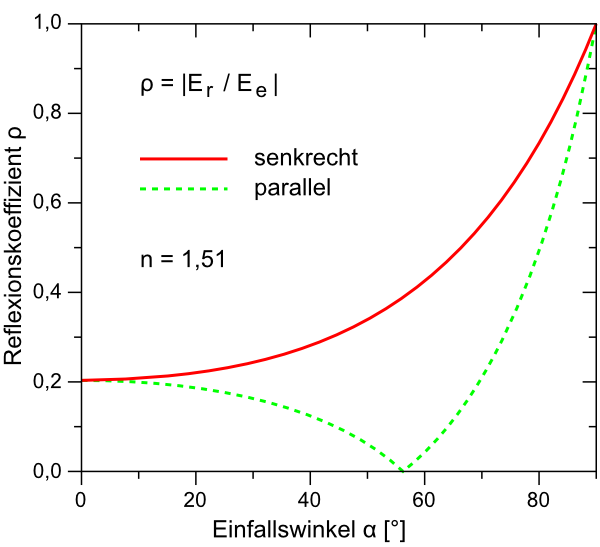
\includegraphics{fresnelkoeff_lp}
	\caption{Reflektionskoeffizienten aufgetragen gegen den Einfallswinkel nach \cite[28.3.2015, 15 Uhr]{lp20}.}
	\label{fig:reflektion}
\end{figure}


\subsection{Brewsterwinkel}
Laut Gleichung \eqref{eq:rp} verschwindet die Reflektion der parallelen Polarisation (s. Grafik \ref{fig:reflektion} falls $\alpha+\beta=45^\circ$, da dann $\tan 45^\circ = \infty$ ist.
Mit Snellnius ergibt sich als Bedingung für $\alpha$:
\begin{align}
	\alpha_B=\arctan\frac{n_2}{n_1}\, .
\end{align}
Diesen Winkel nennt man \textit{Brewster-Winkel}.
Als Erklärung hierfür kann man die Atome als Hertzsche Dipole interpretieren, welche auch nicht in alle Richtungen strahlt.



\subsection{Doppelbrechung}
Doppelbrechende Kristalle sind spezielle Stoffe, welche eine optische Achse besitzen.
Der Brechungsindex parallel und senkrecht zu dieser Achse ist jedoch unterschiedlich.
Trifft ein Strahl auf so einen Kristall, so wird der ordentliche Strahl (derjenige, der senkrecht zur optischen Achse ist) nach dem Snellnius'schen Brechungsgesetz von Gleichung \eqref{eq:snellnius} gebrochen.
Der andere Teil verhält sich anders und wird zum Beispiel auch bei senkrechtem Einfall gebrochen.
Weitere Informationen findet man zum Beispiel in \cite[S. 251]{demtroeder2}.

Dieses Prinzip wird zum Beispiel in einem \textit{Nicol}-Prisma verwendet.
Der Aufbau aus Grafik \ref{fig:nicol} lässt nur eine Polarisation durch das Prisma fallen, während der Rest in andere Richtungen reflektiert und dann absorbiert wird.
\begin{figure}[h]
	\centering
	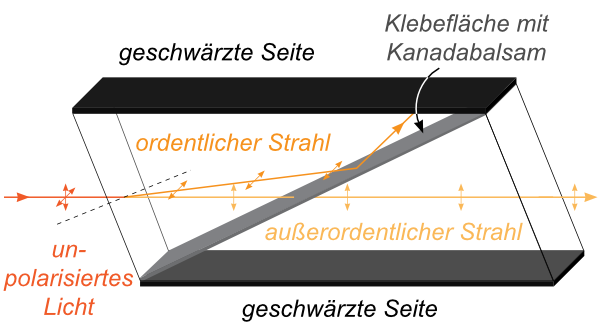
\includegraphics{nicol}
	\caption{Aufbau eines Nicol-Prismas von \cite[28.3.2015, 11 Uhr]{lp20}}
	\label{fig:nicol}
\end{figure}

\section{Durchführung}
\label{sec:durchfuehrung}
Für den Versuch wird eine optische Schiene wie in Abb. \ref{fig:schiene} verwendet, welche sich am Anfang gerade auf $0^\circ $  befindet.
Nachdem die Quecksilberdampflampe angeschaltet wurde und die Intensität ausreicht, kann nun begonnen werden, den Strahlengang einzustellen.
Die sich auf der Schiene befindenden Linsen müssen zunächst ohne das Prisma so abgestimmt werden, dass das (nach dem Filter grüne) Lichtbündel scharf in dem Okular erkennbar ist.
Dafür werden Polarisator und Analysator so eingestellt, dass sie alles Licht durchlassen.
Um die Polarisationsrichtung korrekt einzustellen wird nun das Nicol-Prisma auf den Drehteller gestellt.
Die Standfläche ist dabei so ausgerichtet, dass die optische Achse vertikal zur Strahlrichtung liegt.
Ohne den Analysator im Strahlengang wird nun der Polarisator auf maximalen Durchlass gestellt.


%Da das menschliche Auge Helligkeitsunterschiede wesentlich deutlicher wahrnimmt, wenn die Gesamthelligkeit gering ist, empfielt es sich, zunächst den Punkt der absoluten Dunkelheit zu suchen und dann den Polarisator um $90^\circ$ zu verdrehen.
Für die erste Messung wird nun der Polarisator so eingestellt, dass keine Helligkeit mehr sichtbar ist (was einer Polarisation parallel zur Einfallsebene entspricht) und dann um $45^\circ$ verdreht.
Nun wird das Nicol-Prisma durch ein Glasprisma ersetzt, welches in der $0^\circ$-Lage der Schiene genau im und parallel zum Strahlengang steht.
Auf den Drehtellern befinden sich zumeist schon Markierungen, welche  dadurch überprüft werden können, dass der Strahl bis zu einer Auslenkung von $90^\circ$ der optischen Schiene durch das Okular sichtbar sein muss.

Um nun den Reflektionskoeffizienten zu vermessen wird nun der Analysator erneut in den Strahlengang gestellt.
Er wird nun, während die Schiene in je $5^\circ$-Schritten weiter gestellt wird, in die Position gestellt, dass kein Licht mehr durchgelassen wird.
Die beiden Winkel werden notiert.

Zur Ermittlung des Brewster-Winkels werden nun der Polarisator wieder um $45^\circ$ zurück gedreht und der Analysator entfernt.
Dann wird der Auslenkwinkel der Schiene gesucht und notiert, bei welcher die geringste Intensität zu sehen ist.
Hierbei empfielt es sich, abwechseld mit dem Versuchspartner die Messung durchzuführen.


\begin{figure}[h]
	\centering
	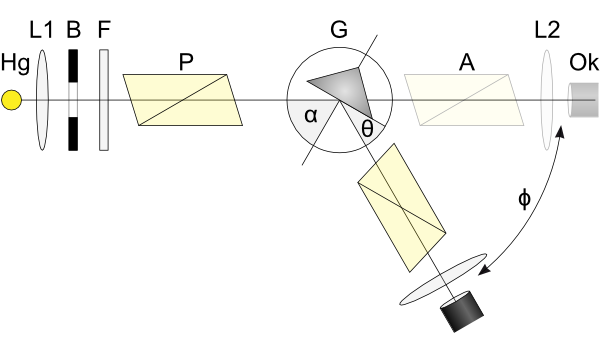
\includegraphics{aufbau}
	\caption{Aufbau des Versuchs von \cite[25.3.2015, 15 Uhr]{lp20}.}
	\label{fig:schiene}
\end{figure}

\section{Auswertung}
\label{sec:auswertung}
Bei dem Versuch ist stets $n_1 =1$ der Brechungsindex der Luft und $n=1.51\pm 0.01$ der Literaturwert des Prismas, welcher vermessen werden soll.
Da der Drehteller mit dem Prisma sich bei der Auslenkung des Hebelarms um den halben Winkel dreht, muss zunächst der gemessene Winkel $\Phi$ umgerechnet werden in den tatsächlichen:
\begin{align*}
	\alpha = 90^\circ - \frac{\Phi}{2}\, .
\end{align*}

\subsection{Drehung der Schwingungsebene}
Der von der Lampe ausgesandte Strahl ist nicht polarisiert.
Ein Nicol-Prisma polarisiert es jedoch in einer bestimmten Ebene.
Diese ist durch die Formel 
\begin{align}
	\tan (\gamma +45^\circ)=\frac{r_s}{r_p}=\frac{\cos(\alpha-\beta)}{\cos (\alpha +\beta)}\label{eq:drehung}
\end{align}
bestimmt, welche nach Gleichung \eqref{eq:snellnius} nur von dem Verhältnis der beiden Brechungsindizes abhängt.

Es war keine direkte Bestimmung der Drehungsebene möglich.
Daher konnte sie nur indirekt bestimmt werden, da bei einem Einfallswinkel von $90^\circ$ das Licht nicht gedreht wird, da beide Polarisationsebenen voll reflektiert werden ($\gamma=0^\circ$).

In Abb. \ref{fig:drehung} wird der Drehwinkel, welcher einen Fehler von $0.2^\circ$ aufweist, gegen den Auftreffwinkel, sowie die Theoriekurve mit $n=1.51$ aufgetragen.
Der Fit der Theoriekurve mit variablem $n$ liefert
\begin{align*}
	n=1.405\pm 0.019\quad .
\end{align*}
\begin{figure}[h]
	\centering
	% GNUPLOT: LaTeX picture with Postscript
\begingroup
  \makeatletter
  \providecommand\color[2][]{%
    \GenericError{(gnuplot) \space\space\space\@spaces}{%
      Package color not loaded in conjunction with
      terminal option `colourtext'%
    }{See the gnuplot documentation for explanation.%
    }{Either use 'blacktext' in gnuplot or load the package
      color.sty in LaTeX.}%
    \renewcommand\color[2][]{}%
  }%
  \providecommand\includegraphics[2][]{%
    \GenericError{(gnuplot) \space\space\space\@spaces}{%
      Package graphicx or graphics not loaded%
    }{See the gnuplot documentation for explanation.%
    }{The gnuplot epslatex terminal needs graphicx.sty or graphics.sty.}%
    \renewcommand\includegraphics[2][]{}%
  }%
  \providecommand\rotatebox[2]{#2}%
  \@ifundefined{ifGPcolor}{%
    \newif\ifGPcolor
    \GPcolortrue
  }{}%
  \@ifundefined{ifGPblacktext}{%
    \newif\ifGPblacktext
    \GPblacktexttrue
  }{}%
  % define a \g@addto@macro without @ in the name:
  \let\gplgaddtomacro\g@addto@macro
  % define empty templates for all commands taking text:
  \gdef\gplbacktext{}%
  \gdef\gplfronttext{}%
  \makeatother
  \ifGPblacktext
    % no textcolor at all
    \def\colorrgb#1{}%
    \def\colorgray#1{}%
  \else
    % gray or color?
    \ifGPcolor
      \def\colorrgb#1{\color[rgb]{#1}}%
      \def\colorgray#1{\color[gray]{#1}}%
      \expandafter\def\csname LTw\endcsname{\color{white}}%
      \expandafter\def\csname LTb\endcsname{\color{black}}%
      \expandafter\def\csname LTa\endcsname{\color{black}}%
      \expandafter\def\csname LT0\endcsname{\color[rgb]{1,0,0}}%
      \expandafter\def\csname LT1\endcsname{\color[rgb]{0,1,0}}%
      \expandafter\def\csname LT2\endcsname{\color[rgb]{0,0,1}}%
      \expandafter\def\csname LT3\endcsname{\color[rgb]{1,0,1}}%
      \expandafter\def\csname LT4\endcsname{\color[rgb]{0,1,1}}%
      \expandafter\def\csname LT5\endcsname{\color[rgb]{1,1,0}}%
      \expandafter\def\csname LT6\endcsname{\color[rgb]{0,0,0}}%
      \expandafter\def\csname LT7\endcsname{\color[rgb]{1,0.3,0}}%
      \expandafter\def\csname LT8\endcsname{\color[rgb]{0.5,0.5,0.5}}%
    \else
      % gray
      \def\colorrgb#1{\color{black}}%
      \def\colorgray#1{\color[gray]{#1}}%
      \expandafter\def\csname LTw\endcsname{\color{white}}%
      \expandafter\def\csname LTb\endcsname{\color{black}}%
      \expandafter\def\csname LTa\endcsname{\color{black}}%
      \expandafter\def\csname LT0\endcsname{\color{black}}%
      \expandafter\def\csname LT1\endcsname{\color{black}}%
      \expandafter\def\csname LT2\endcsname{\color{black}}%
      \expandafter\def\csname LT3\endcsname{\color{black}}%
      \expandafter\def\csname LT4\endcsname{\color{black}}%
      \expandafter\def\csname LT5\endcsname{\color{black}}%
      \expandafter\def\csname LT6\endcsname{\color{black}}%
      \expandafter\def\csname LT7\endcsname{\color{black}}%
      \expandafter\def\csname LT8\endcsname{\color{black}}%
    \fi
  \fi
  \setlength{\unitlength}{0.0500bp}%
  \begin{picture}(7200.00,5040.00)%
    \gplgaddtomacro\gplbacktext{%
      \csname LTb\endcsname%
      \put(814,704){\makebox(0,0)[r]{\strut{}-10}}%
      \put(814,1213){\makebox(0,0)[r]{\strut{} 0}}%
      \put(814,1722){\makebox(0,0)[r]{\strut{} 10}}%
      \put(814,2231){\makebox(0,0)[r]{\strut{} 20}}%
      \put(814,2740){\makebox(0,0)[r]{\strut{} 30}}%
      \put(814,3248){\makebox(0,0)[r]{\strut{} 40}}%
      \put(814,3757){\makebox(0,0)[r]{\strut{} 50}}%
      \put(814,4266){\makebox(0,0)[r]{\strut{} 60}}%
      \put(814,4775){\makebox(0,0)[r]{\strut{} 70}}%
      \put(946,484){\makebox(0,0){\strut{} 40}}%
      \put(2011,484){\makebox(0,0){\strut{} 50}}%
      \put(3076,484){\makebox(0,0){\strut{} 60}}%
      \put(4141,484){\makebox(0,0){\strut{} 70}}%
      \put(5206,484){\makebox(0,0){\strut{} 80}}%
      \put(6271,484){\makebox(0,0){\strut{} 90}}%
      \put(176,2739){\rotatebox{-270}{\makebox(0,0){\strut{}Drehwinkel $\gamma$ [$^\circ$]}}}%
      \put(3874,154){\makebox(0,0){\strut{}Auftreffwinkel $\alpha$ [$^\circ$]}}%
    }%
    \gplgaddtomacro\gplfronttext{%
      \csname LTb\endcsname%
      \put(5816,4602){\makebox(0,0)[r]{\strut{}Messwerte}}%
      \csname LTb\endcsname%
      \put(5816,4382){\makebox(0,0)[r]{\strut{}Theoriekurve}}%
      \csname LTb\endcsname%
      \put(5816,4162){\makebox(0,0)[r]{\strut{}Theorie gefittet}}%
    }%
    \gplbacktext
    \put(0,0){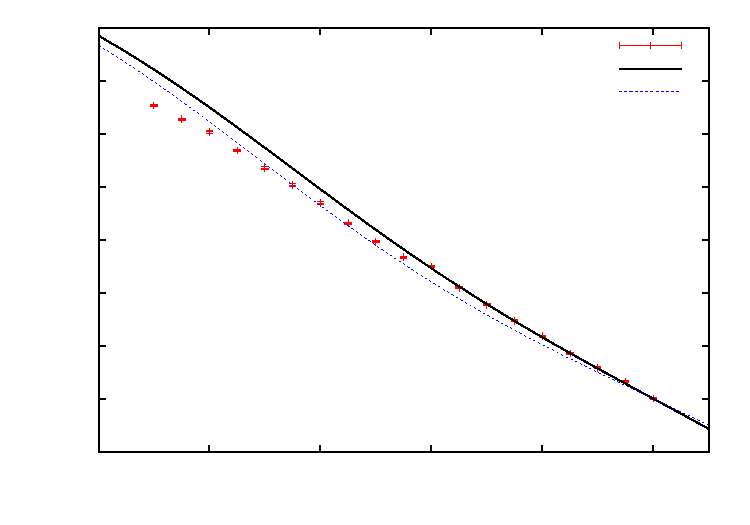
\includegraphics{drehung}}%
    \gplfronttext
  \end{picture}%
\endgroup

	\caption{Drehwinkel $\gamma$ gegen den Auftreffwinkel $\alpha$ aufgetragen.}
	\label{fig:drehung}
\end{figure}

\subsection{Brechungsindex bei $\gamma=45^\circ$}
Der Brewsterwinkel $\alpha_B$ liegt gerade bei einem Drehwinkel von $\gamma=45^\circ$, da dort laut Gleichung \eqref{eq:drehung} $\cos (\alpha + \beta) = 0 \Rightarrow \alpha + \beta = 90^\circ$ ist.
In Abb. \ref{fig:brewster} sind die umliegenden Werte aufgetragen, so dass mit Hilfe einer linearen Regression der Brewsterwinkel bestimmt werden kann.
Die so ermittelte Geradensteigung ist $m=-1.283\pm 0.029$ und der $y$-Achsenabschnitt beträgt $b=(114.1\pm 1.6)^\circ$.
Die daraus berechnete Gerade beträgt damit
\begin{align}
	\alpha_B&=\frac{b-45^\circ}{m} = (53.8\pm 1.8)^\circ\\
	\sigma_{\alpha_B}&=\sqrt{\left( \frac{\sigma_b}{m} \right)^2 + \left( \frac{\sigma_m(b-45^\circ)}{m^2} \right)^2}
\end{align}
wobei sich der Fehler nach der Gaußschen Fehlerfortpflanzung berechnet.
Der Brechungsindex, der sich daraus ergibt, hat einen Fehler von
\begin{align*}
	\sigma_n=\frac{\sigma_\alpha}{\cos ^2\alpha}
\end{align*}
und beträgt 
\begin{align}
	n=1.37\pm 0.10\, .
\end{align}



\begin{figure}[h]
	\centering
	% GNUPLOT: LaTeX picture with Postscript
\begingroup
  \makeatletter
  \providecommand\color[2][]{%
    \GenericError{(gnuplot) \space\space\space\@spaces}{%
      Package color not loaded in conjunction with
      terminal option `colourtext'%
    }{See the gnuplot documentation for explanation.%
    }{Either use 'blacktext' in gnuplot or load the package
      color.sty in LaTeX.}%
    \renewcommand\color[2][]{}%
  }%
  \providecommand\includegraphics[2][]{%
    \GenericError{(gnuplot) \space\space\space\@spaces}{%
      Package graphicx or graphics not loaded%
    }{See the gnuplot documentation for explanation.%
    }{The gnuplot epslatex terminal needs graphicx.sty or graphics.sty.}%
    \renewcommand\includegraphics[2][]{}%
  }%
  \providecommand\rotatebox[2]{#2}%
  \@ifundefined{ifGPcolor}{%
    \newif\ifGPcolor
    \GPcolortrue
  }{}%
  \@ifundefined{ifGPblacktext}{%
    \newif\ifGPblacktext
    \GPblacktexttrue
  }{}%
  % define a \g@addto@macro without @ in the name:
  \let\gplgaddtomacro\g@addto@macro
  % define empty templates for all commands taking text:
  \gdef\gplbacktext{}%
  \gdef\gplfronttext{}%
  \makeatother
  \ifGPblacktext
    % no textcolor at all
    \def\colorrgb#1{}%
    \def\colorgray#1{}%
  \else
    % gray or color?
    \ifGPcolor
      \def\colorrgb#1{\color[rgb]{#1}}%
      \def\colorgray#1{\color[gray]{#1}}%
      \expandafter\def\csname LTw\endcsname{\color{white}}%
      \expandafter\def\csname LTb\endcsname{\color{black}}%
      \expandafter\def\csname LTa\endcsname{\color{black}}%
      \expandafter\def\csname LT0\endcsname{\color[rgb]{1,0,0}}%
      \expandafter\def\csname LT1\endcsname{\color[rgb]{0,1,0}}%
      \expandafter\def\csname LT2\endcsname{\color[rgb]{0,0,1}}%
      \expandafter\def\csname LT3\endcsname{\color[rgb]{1,0,1}}%
      \expandafter\def\csname LT4\endcsname{\color[rgb]{0,1,1}}%
      \expandafter\def\csname LT5\endcsname{\color[rgb]{1,1,0}}%
      \expandafter\def\csname LT6\endcsname{\color[rgb]{0,0,0}}%
      \expandafter\def\csname LT7\endcsname{\color[rgb]{1,0.3,0}}%
      \expandafter\def\csname LT8\endcsname{\color[rgb]{0.5,0.5,0.5}}%
    \else
      % gray
      \def\colorrgb#1{\color{black}}%
      \def\colorgray#1{\color[gray]{#1}}%
      \expandafter\def\csname LTw\endcsname{\color{white}}%
      \expandafter\def\csname LTb\endcsname{\color{black}}%
      \expandafter\def\csname LTa\endcsname{\color{black}}%
      \expandafter\def\csname LT0\endcsname{\color{black}}%
      \expandafter\def\csname LT1\endcsname{\color{black}}%
      \expandafter\def\csname LT2\endcsname{\color{black}}%
      \expandafter\def\csname LT3\endcsname{\color{black}}%
      \expandafter\def\csname LT4\endcsname{\color{black}}%
      \expandafter\def\csname LT5\endcsname{\color{black}}%
      \expandafter\def\csname LT6\endcsname{\color{black}}%
      \expandafter\def\csname LT7\endcsname{\color{black}}%
      \expandafter\def\csname LT8\endcsname{\color{black}}%
    \fi
  \fi
  \setlength{\unitlength}{0.0500bp}%
  \begin{picture}(7200.00,5040.00)%
    \gplgaddtomacro\gplbacktext{%
      \csname LTb\endcsname%
      \put(814,704){\makebox(0,0)[r]{\strut{} 30}}%
      \put(814,1286){\makebox(0,0)[r]{\strut{} 35}}%
      \put(814,1867){\makebox(0,0)[r]{\strut{} 40}}%
      \put(814,2449){\makebox(0,0)[r]{\strut{} 45}}%
      \put(814,3030){\makebox(0,0)[r]{\strut{} 50}}%
      \put(814,3612){\makebox(0,0)[r]{\strut{} 55}}%
      \put(814,4193){\makebox(0,0)[r]{\strut{} 60}}%
      \put(814,4775){\makebox(0,0)[r]{\strut{} 65}}%
      \put(946,484){\makebox(0,0){\strut{} 46}}%
      \put(1727,484){\makebox(0,0){\strut{} 48}}%
      \put(2508,484){\makebox(0,0){\strut{} 50}}%
      \put(3289,484){\makebox(0,0){\strut{} 52}}%
      \put(4070,484){\makebox(0,0){\strut{} 54}}%
      \put(4851,484){\makebox(0,0){\strut{} 56}}%
      \put(5632,484){\makebox(0,0){\strut{} 58}}%
      \put(6413,484){\makebox(0,0){\strut{} 60}}%
      \put(176,2739){\rotatebox{-270}{\makebox(0,0){\strut{}Drehwinkel $\gamma$ [$^\circ$]}}}%
      \put(3874,154){\makebox(0,0){\strut{}Auftreffwinkel $\alpha$ [$^\circ$]}}%
    }%
    \gplgaddtomacro\gplfronttext{%
      \csname LTb\endcsname%
      \put(5816,4602){\makebox(0,0)[r]{\strut{}Messwerte}}%
      \csname LTb\endcsname%
      \put(5816,4382){\makebox(0,0)[r]{\strut{}lineare Regression}}%
      \csname LTb\endcsname%
      \put(5816,4162){\makebox(0,0)[r]{\strut{}Theorie gefittet}}%
      \csname LTb\endcsname%
      \put(5816,3942){\makebox(0,0)[r]{\strut{}Theoriekurve}}%
      \csname LTb\endcsname%
      \put(5816,3722){\makebox(0,0)[r]{\strut{}Brewster-Winkel}}%
    }%
    \gplbacktext
    \put(0,0){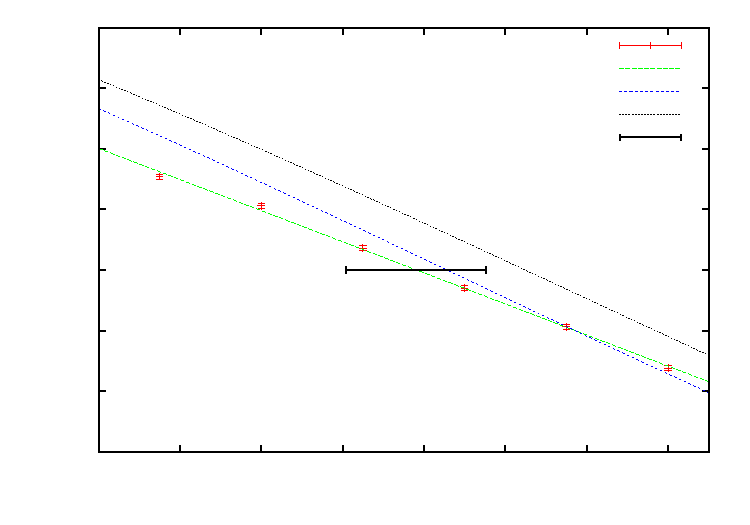
\includegraphics{drehung_zoom}}%
    \gplfronttext
  \end{picture}%
\endgroup

	\caption{Ausschnitt aus Abb. \ref{fig:drehung} zur Bestimmung des Brewsterwinkels.}
	\label{fig:brewster}
\end{figure}

\subsection{Brewsterwinkel}
Die Messung des Brewsterwinkels wurde zweimal gemacht: die ersten 6 Werte wurden mit unverstelltem Polarisator gemacht.
Da dabei das Minimum nicht scharf zu sehen war, wurde danach der Polarisator um ca. $5^\circ$ verdreht, wodurch die Messung erheblich genauer wurde.
Hiermit wurden 4 Werte aufgezeichnet.
Diese können nun auf verschiedene Weise ausgewertet werden: die einzelnen Messreihen und die einzelnen Versuchspartner.

In Tabelle \ref{tab:brewster} sind die Werte eingetragen.
Aus dem Literaturwert des Brehungsindexes von $n=1.51\pm 0.01$ kann der theoretische Brewsterwinkel berechnet werden: er liegt bei
\begin{align}
	\alpha_B=\arctan \frac{n}{n_1}\approx 56.49^\circ
\end{align}
\begin{table}[!htb]
\centering
\begin{tabular}{|c|c|c|c|}
         \hline
         & $\Phi_B$ [$^\circ$] & $\alpha_B$ [$^\circ$] & $n$ \\
         \hline
         Alle Werte & $66.6 \pm 0.6$ & $56.7 \pm 0.3$ & $1.522 \pm 0.018$ \\
         Messreihe 1& $66.4 \pm 0.9$ & $56.8 \pm 0.5$ & $1.53 \pm 0.03$ \\
         Messreihe 2& $67.0 \pm 0.5$ & $56.50 \pm 0.25$ & $1.511 \pm 0.015$ \\
         \hline
         Felix & $65.9 \pm 1.0$ & $57.1 \pm 0.5$ & $1.55 \pm 0.03$ \\
         Michael & $67.3 \pm 0.5$ & $56.35 \pm 0.25$ & $1.502 \pm 0.015$ \\
         \hline
\end{tabular}
\caption{Bestimmung des Brewsterwinkels.}
\label{tab:brewster}
\end{table}



\section{Diskussion}
\label{sec:diskussion}
\subsection{Drehung der Schwingungsebene}
In Abbildung \ref{fig:drehung} ist ein klarer Sprung bei einem Auslenkwinkel von $\alpha=70^\circ$ in der Kurve zu erkennen.
Dieser könnte dadurch hervorgerufen worden sein, dass die ersten Werte alle um $5^\circ$ zu niedrig abgelesen wurden.
An einer Stelle war auch in den Daten schon ein Sprung zu sehen, den wir jedoch nicht weiter untersucht haben.
Allerdings könnte auch ein verrutschtes Prisma dies hervorrufen.
Betrachtet man die Daten nach dem Sprung, so stimmen diese sehr genau mit der Theoriekurve überein.

Die Bestimmung des Brewsterwinkels aus der Drehung der Schwingungsebene ist wie zu erwarten sehr ungenau, da dieser vor dem Sprung liegt.
Dennoch ist er nur um 5\% kleiner als der Theoriewert, auch wenn das Fehlerintervall diesen nicht schneidet.



\subsection{Brewsterwinkel}
Bei der Messung des Brewsterwinkels fällt auf, dass die Werte, welche mit dem verstellten Polarisator gemessen wurden, deutlich genauer sind, als die anderen.
Dies kommt dadurch zu stande, dass das Intensitätsminimum deutlicher zu sehen war.
Für zukünftige Versuchsdurchführungen ist es desshalb ebenfalls zu empfehlen, zunächst ungefähr den Brewsterwinkel zu suchen und dann den Polarisator noch nachzujustieren.

Auch zwischen den beiden Versuchspartnern sind deutliche Unterschiede zu erkennen.
Dies ist dadurch zu erklären, dass die Helligkeitsunterschiede nicht groß waren und dass (zumindest so der subjektive Eindruck) auch mehrere dunkle Bereiche zu erkennen waren.
Es erforderte also einige Übung, den richtigen zu finden.


\subsection{Brechungsindex}
Der gemittelte gewichtete Brechungsindex aller Messungen beträgt $n = 1.465 \pm 0.013$ und ist damit um $3 \%$ kleiner, als der Literaturwert mit $n=1.51\pm 0.01$.
Auch das Fehlerintervall schließt diesen nicht mit ein.
Dennoch sind die Werte in der richtigen Größenordnung und für die beschriebenen Fehlerquellen sehr gut.



\bibliography{literatur} 
\bibliographystyle{babalpha} 
\end{document}
